\documentclass[12pt]{article}
\title{ECE 3 Lab 3 PreLab}

\author{Lawrence Liu}
\usepackage{graphicx}
\usepackage{amsmath}
\setlength{\parindent}{0pt}
\usepackage[section]{placeins}
\begin{document}
\maketitle

\section*{Problem 1}
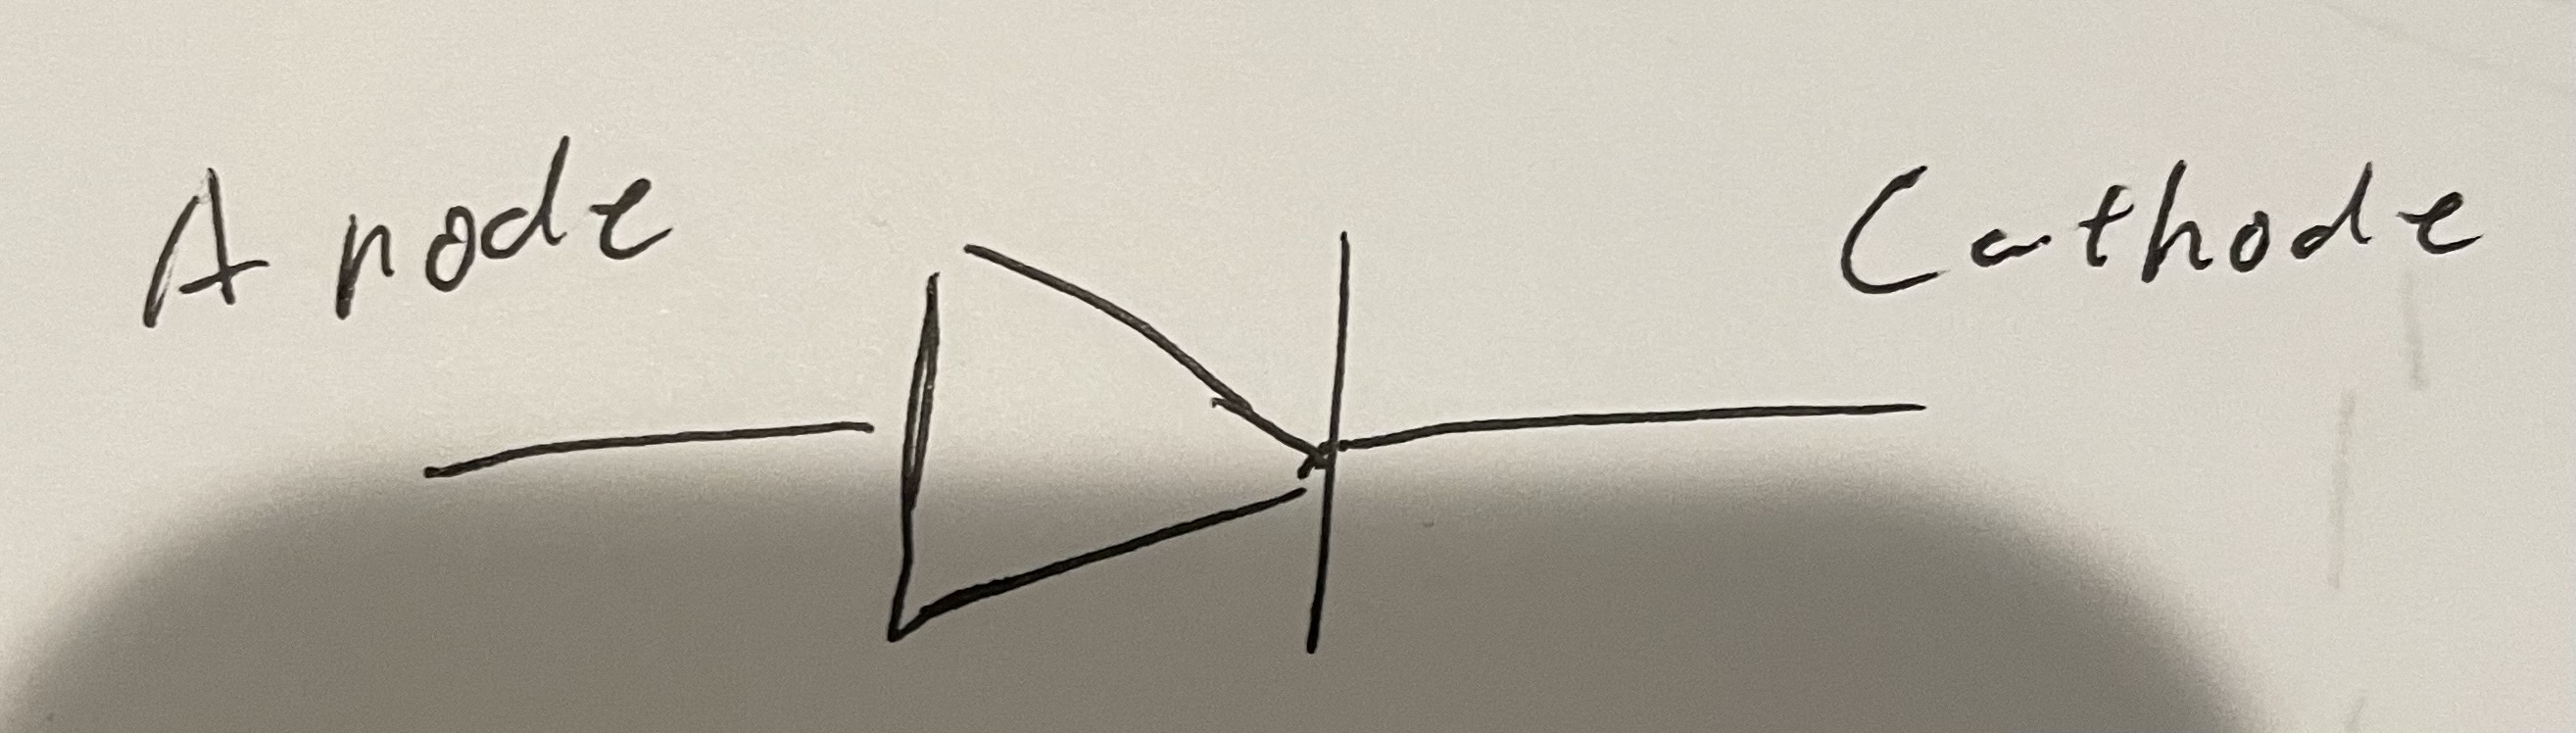
\includegraphics[scale=0.5]{Diode}
\section*{Problem 2}
Higher
\section*{Problem 3}
Look at the length of the leads or look at the size of the metal plates inside of the LED
\section*{Problem 4}

\section*{Problem 5}
$\frac{1}{s}$ because the units of $RC$ is $F\Omega=\frac{1}{s}$
\section*{Problem 6}
\subsection*{Oscilloscope Circuit 1}
Yes, Grounds are shorted
\subsection*{Oscilloscope Circuit 2}
No, Grounds are not shorted, there is a resistor in between. 
\subsection*{Oscilloscope Circuit 2}
Yes, the Battery has no ground
\subsection*{AD2 Circuit 1}
Yes, because of differential probing we don't need to worry about accidentally causing shorts
\subsection*{AD2 Circuit 2}
Yes, because of differential probing we don't need to worry about accidentally causing shorts

\end{document}

